\documentclass[12pt]{article}
\usepackage[utf8]{inputenc}
\usepackage{graphicx}
\usepackage[export]{adjustbox}
\usepackage{caption}
\usepackage{natbib}
\usepackage{refstyle}
\usepackage{float}
\usepackage{hyperref}

\begin{document}
\title{Safe Evolution Templates for Software Product Lines - Catalogue} 
\author{Software Productivity Group}
\date{\today} 
\maketitle


\section{Templates for Compositional Product Lines}

\begin{figure}[H]
\centering
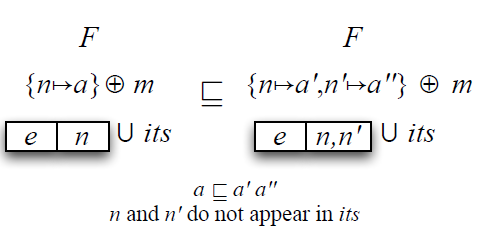
\includegraphics[width=1\textwidth, frame]{images/SplitAsset}
\caption{Split Asset (Taken from \cite{phdlmt})}
\end{figure}

\begin{figure}[H]
\centering
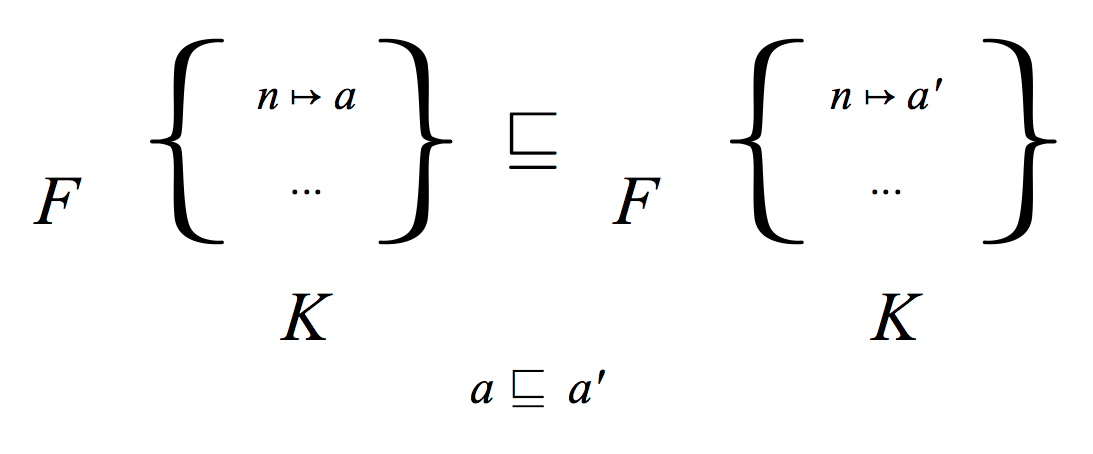
\includegraphics[width=1\textwidth, frame]{images/TemplateRefactorAsset}
\caption{Refine Asset (Taken from \cite{phdlmt})}
\end{figure}

\begin{figure}[H]
\centering
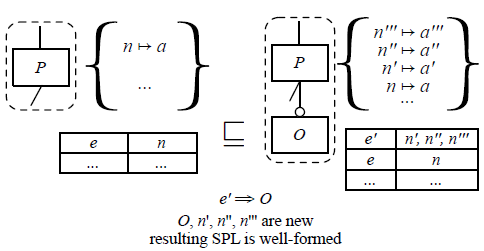
\includegraphics[width=1\textwidth, frame]{images/AddNewOptionalFeature}
\caption{Add New Optional Feature (Taken from \cite{phdlmt})}
\end{figure}

\begin{figure}[H]
\centering
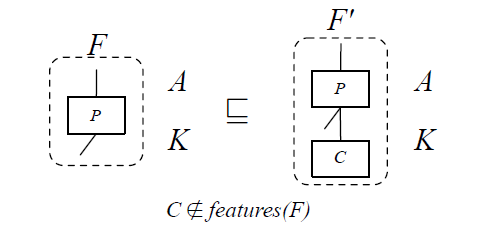
\includegraphics[width=1\textwidth, frame]{images/AddAnyFeatureWithoutImpl}
\caption{Add any feature without changing the AM and CK (Taken from \cite{phdlmt})}
\end{figure}

\begin{figure}[H]
\centering
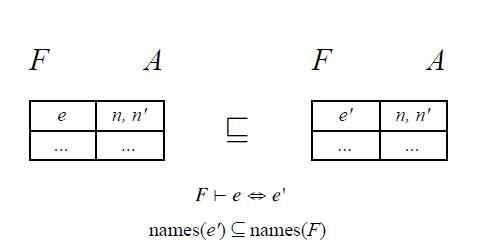
\includegraphics[width=1\textwidth, frame]{images/ReplaceFeatureExpression}
\caption{Replace Feature Expression (Taken from \cite{phdlmt})}
\end{figure}

\begin{figure}[H]
\centering
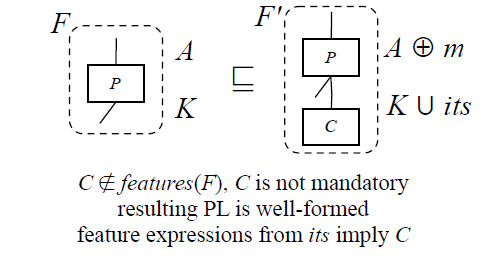
\includegraphics[width=1\textwidth, frame]{images/AddVariableFeatureWithImpl}
\caption{Add variable feature with implementation (Taken from \cite{phdlmt})}
\end{figure}

\begin{figure}[H]
\centering
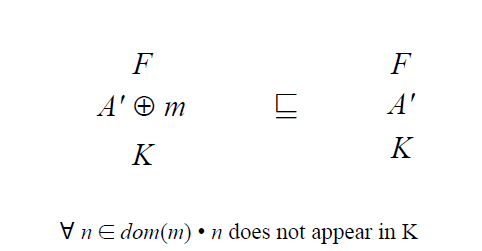
\includegraphics[width=1\textwidth, frame]{images/RemoveUnusedAssets}
\caption{Remove Unused Assets (Taken from \cite{phdlmt})}
\end{figure}

\begin{figure}[H]
\centering
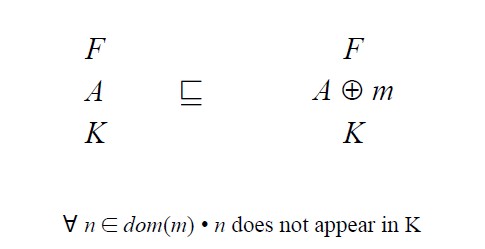
\includegraphics[width=1\textwidth, frame]{images/AddUnusedAssets}
\caption{Add Unused Assets (Taken from \cite{phdlmt})}
\end{figure}

\begin{figure}[H]
\centering
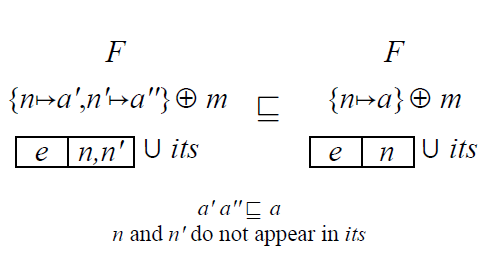
\includegraphics[width=1\textwidth, frame]{images/MergeAssets}
\caption{Merge Assets (Taken from \cite{phdlmt})}
\end{figure}

\begin{figure}[H]
\centering
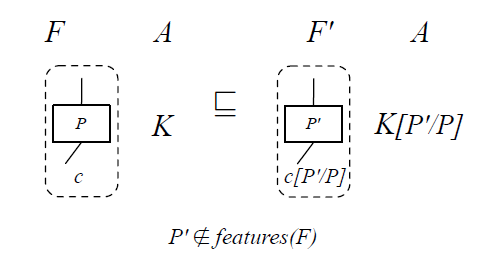
\includegraphics[width=1\textwidth, frame]{images/FeatureRenaming}
\caption{Feature Renaming (Taken from \cite{phdlmt})}
\end{figure}

\begin{figure}[H]
\centering
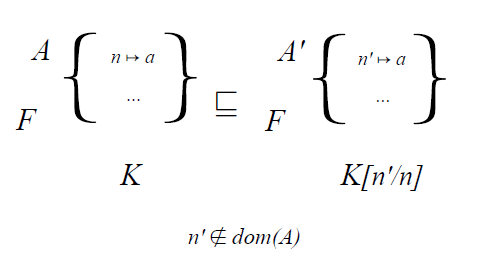
\includegraphics[width=1\textwidth, frame]{images/AssetNameRenaming}
\caption{Asset Name Renaming (Taken from \cite{phdlmt})}
\end{figure}

\begin{figure}[H]
\centering
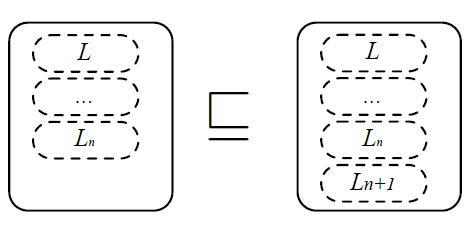
\includegraphics[width=1\textwidth, frame]{images/AddProductLine}
\caption{Add Product Line (Taken from \cite{phdlmt})}
\end{figure}

\begin{figure}[H]
\centering
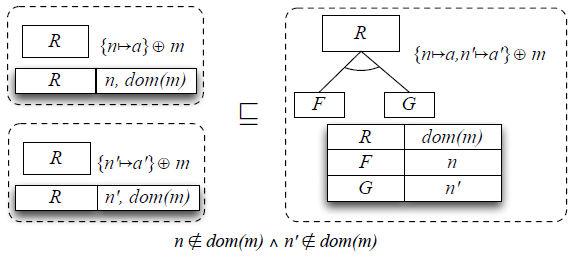
\includegraphics[width=1\textwidth, frame]{images/MergeProductsIntoAPL}
\caption{Merge Products Into a PL (Taken from \cite{phdlmt})}
\end{figure}

\begin{figure}[H]
\centering
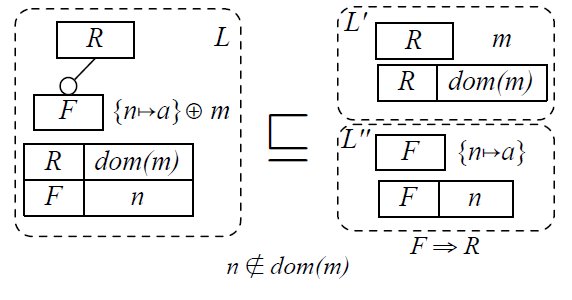
\includegraphics[width=1\textwidth, frame]{images/DeriveMultiProductLine}
\caption{Derive Multi Product Line from a Product Line (Taken from \cite{phdlmt})}
\end{figure}

\pagebreak
\section{Templates for Annotative Product Lines}

\begin{figure}[H]
\centering
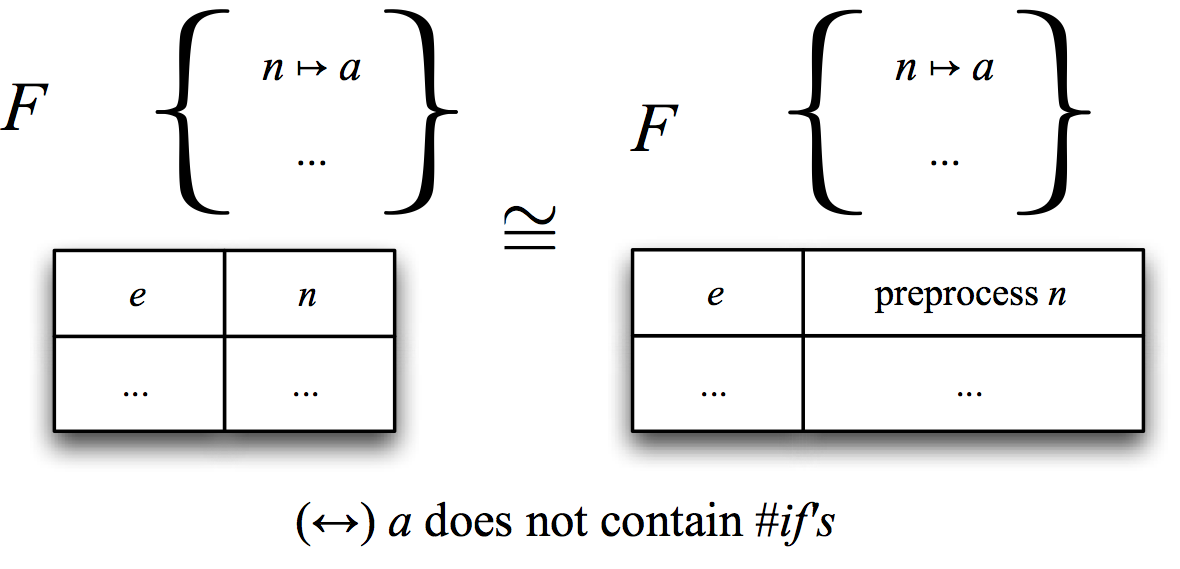
\includegraphics[width=1\textwidth, frame]{images/Template1T}
\caption{Preprocess Asset Without Preprocessor Directive (Taken from \cite{twiki})}
\end{figure}

\begin{figure}[H]
\centering
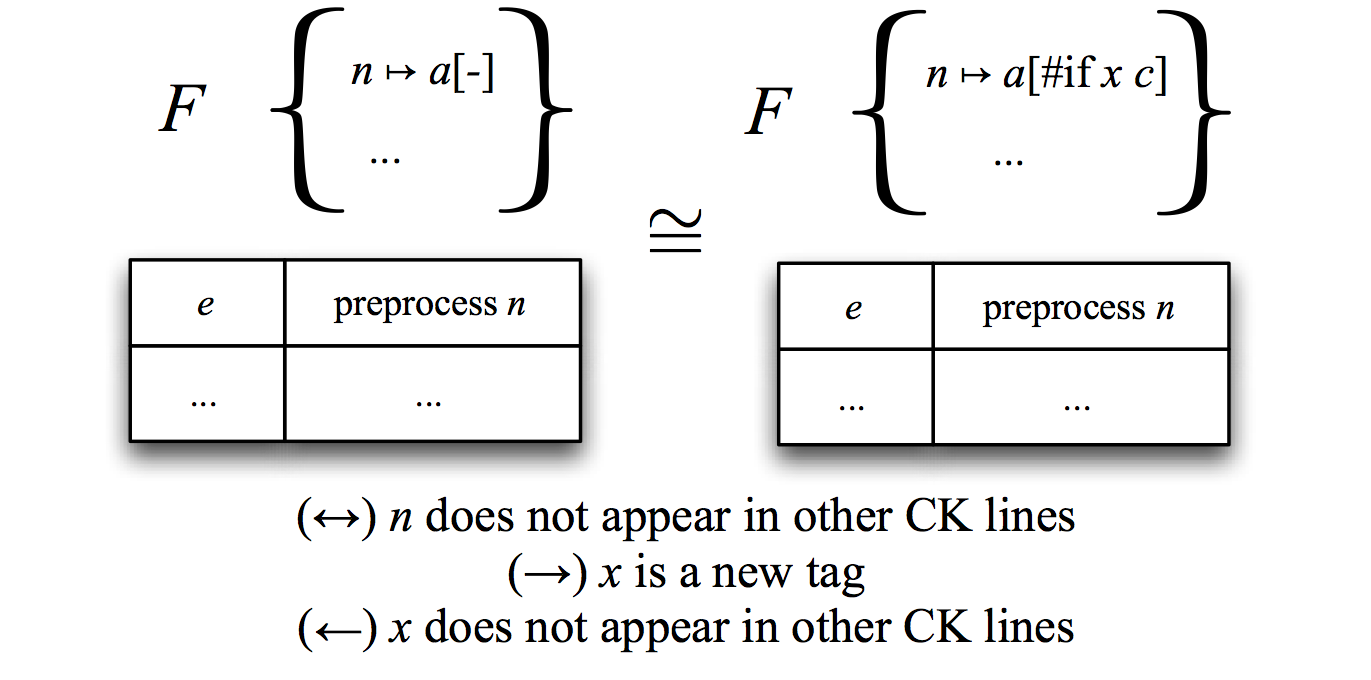
\includegraphics[width=1\textwidth, frame]{images/Template2T}
\caption{Add Dead Preprocessed Code (Taken from \cite{twiki})}
\end{figure}

\begin{figure}[H]
\centering
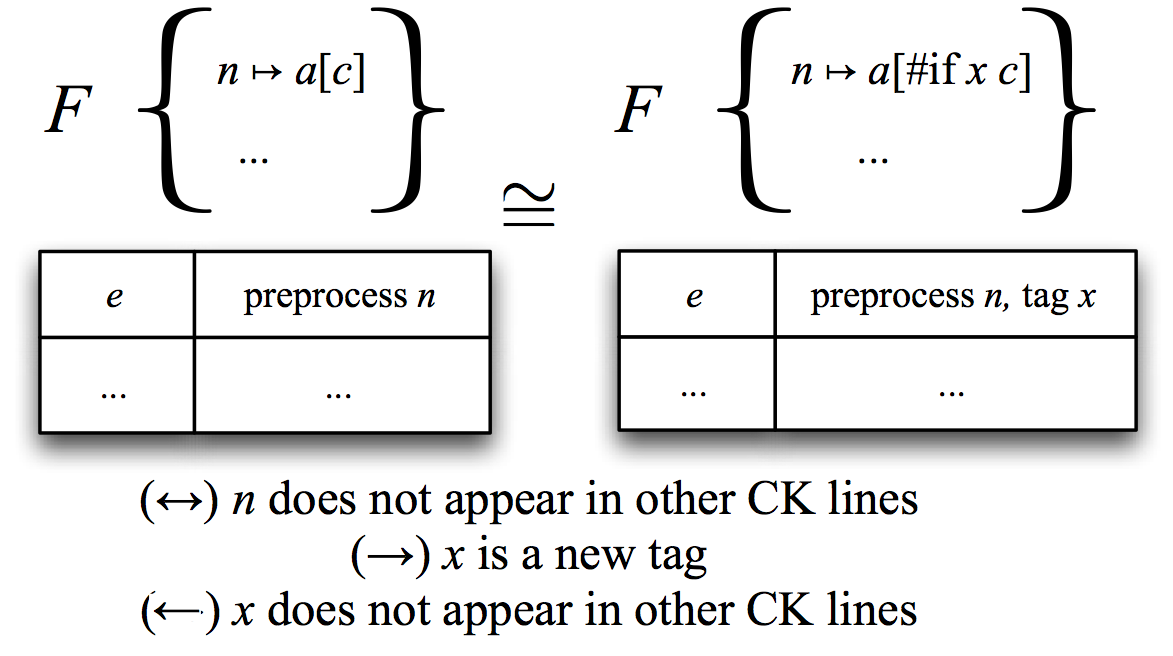
\includegraphics[width=1\textwidth, frame]{images/Template3T}
\caption{Add Harmless Preprocessing Directive (Taken from \cite{twiki})}
\end{figure}

\begin{figure}[H]
\centering
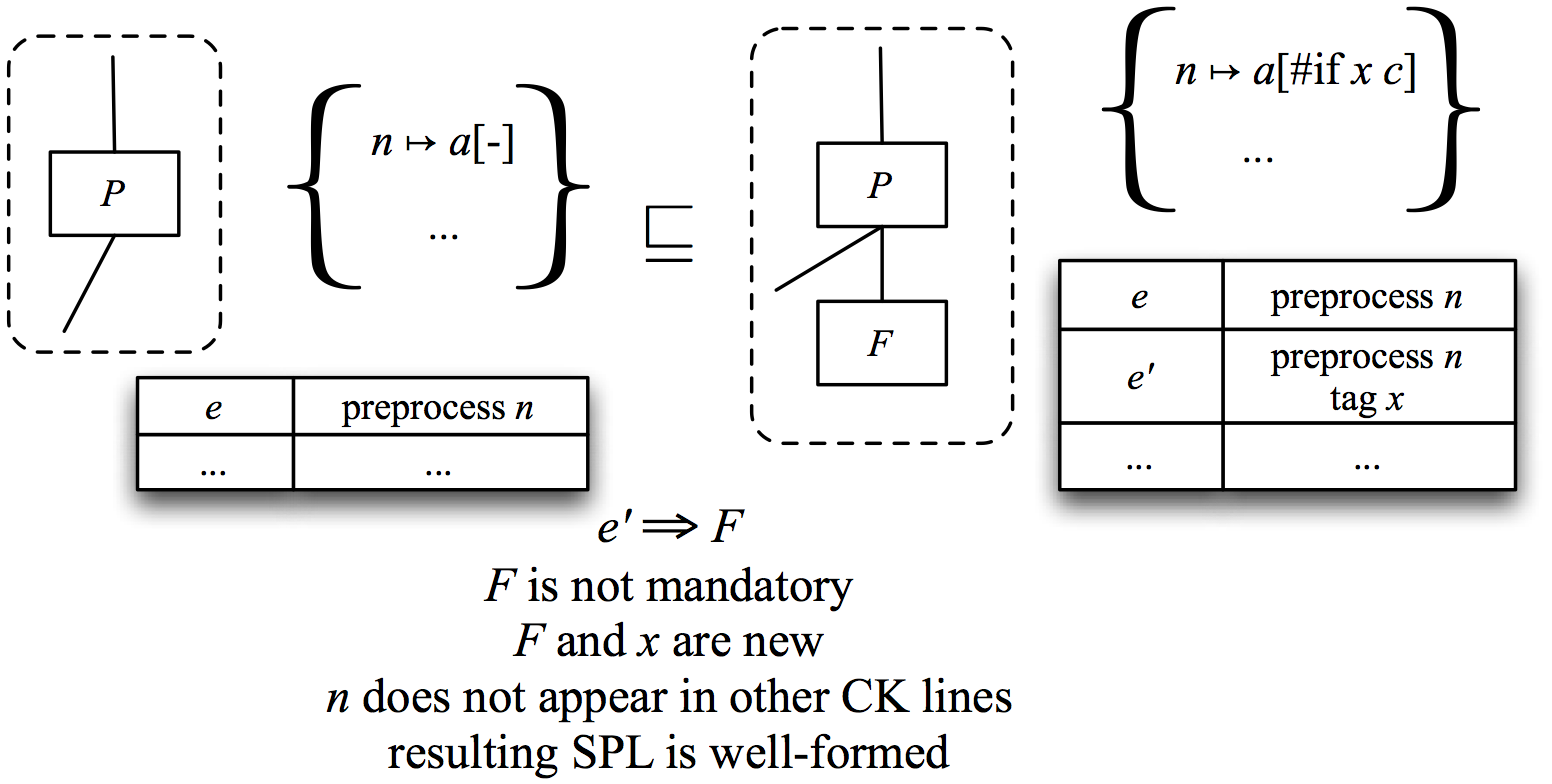
\includegraphics[width=1\textwidth, frame]{images/Template4T}
\caption{Add New Preprocessed Feature (Taken from \cite{twiki})}
\end{figure}

\begin{figure}[H]
\centering
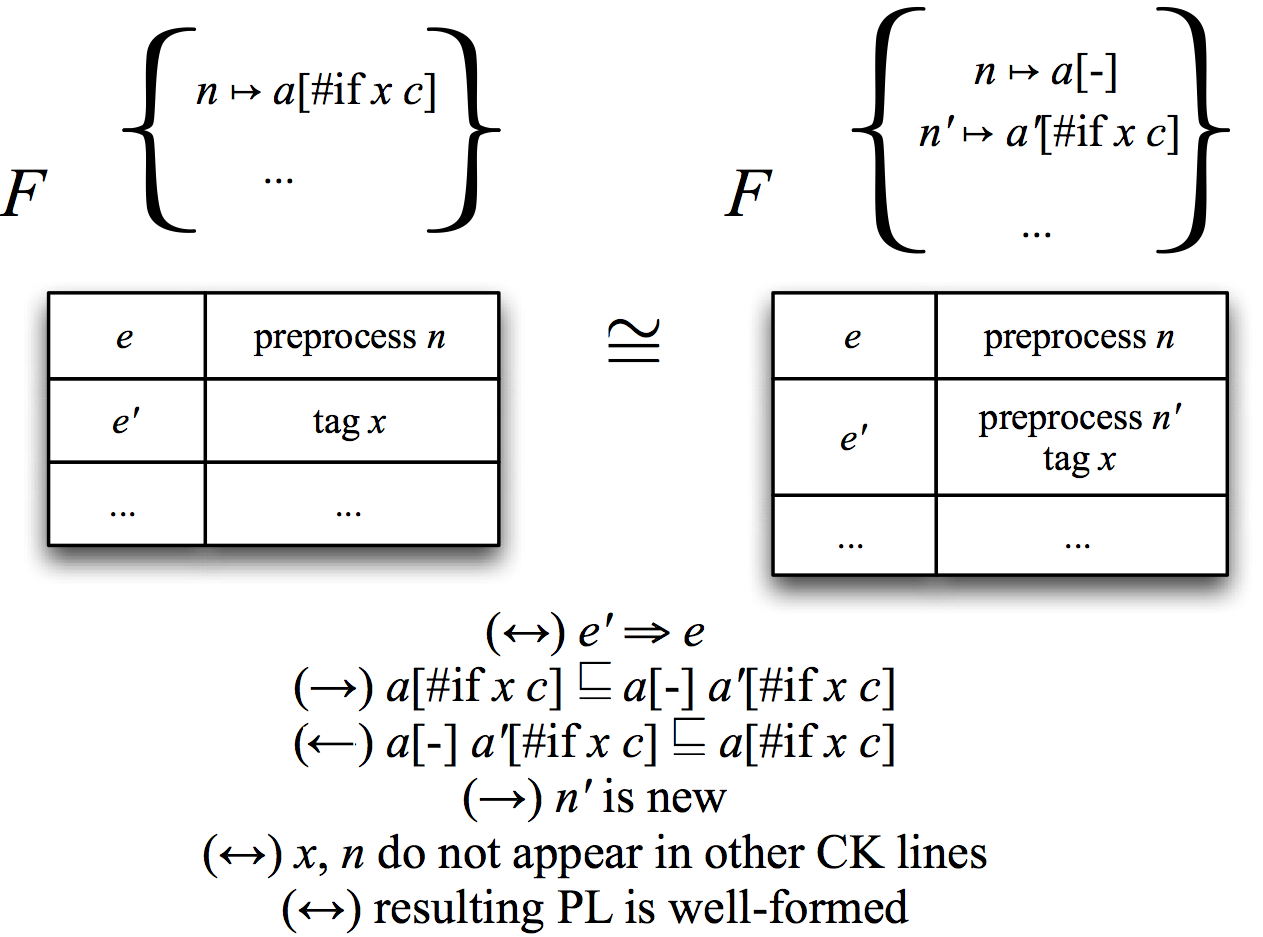
\includegraphics[width=0.9\textwidth, frame]{images/Template5T}
\caption{Extract Preprocessed Code (Taken from \cite{twiki})}
\end{figure}

\begin{figure}[H]
\centering
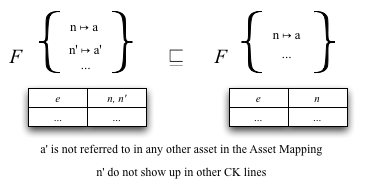
\includegraphics[width=1\textwidth, frame]{images/TemplatesDeleteAsset}
\caption{Delete Asset (Taken from \cite{twiki})}
\end{figure}

\pagebreak
\section{Templates for CK Refactoring}

\begin{figure}[H]
\centering
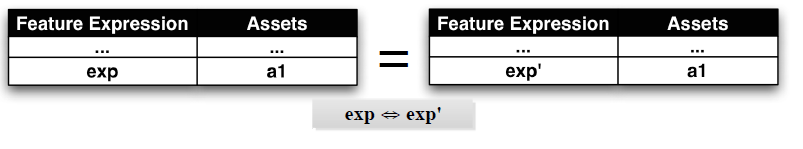
\includegraphics[width=1\textwidth, frame]{images/SimplifyFeatureExpression}
\caption{Simplify Feature Expression using Propositional Reasoning (Taken from \cite{msclmt})}
\end{figure}

\begin{figure}[H]
\centering
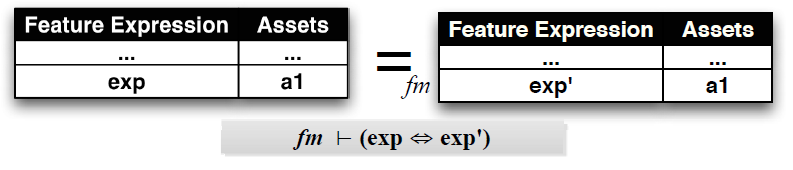
\includegraphics[width=1\textwidth, frame]{images/SimplifyFeatureExpression2}
\caption{Simplify Feature Expression using the FM (Taken from \cite{msclmt})}
\end{figure}

\begin{figure}[H]
\centering
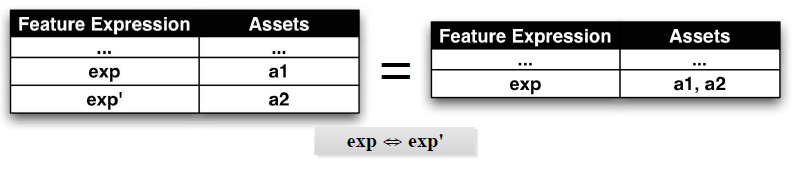
\includegraphics[width=1\textwidth, frame]{images/MergeItems}
\caption{Merge items with propositionally equivalent feature expressions (Taken from \cite{msclmt})}
\end{figure}

\begin{figure}[H]
\centering
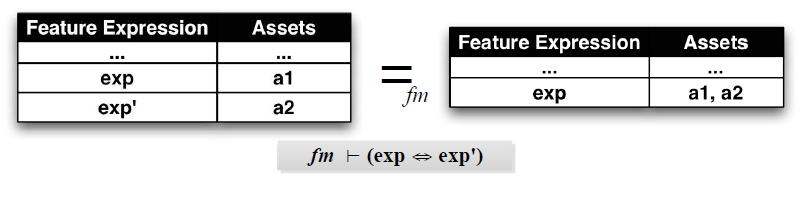
\includegraphics[width=1\textwidth, frame]{images/MergeItems2}
\caption{Merge items with equivalent feature expressions by the FM (Taken from \cite{msclmt})}
\end{figure}

\begin{figure}[H]
\centering
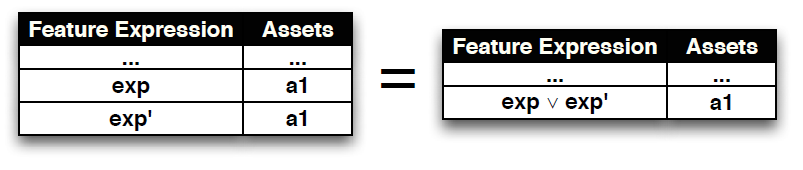
\includegraphics[width=1\textwidth, frame]{images/DuplicatedAssets}
\caption{Duplicated Assets (Taken from \cite{msclmt})}
\end{figure}

\begin{figure}[H]
\centering
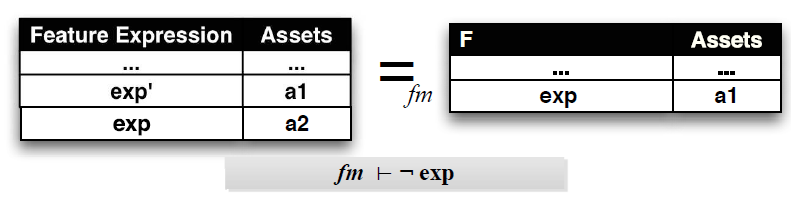
\includegraphics[width=1\textwidth, frame]{images/DeadFeatureExpression}
\caption{Dead Feature Expression (Taken from \cite{msclmt})}
\end{figure}

\begin{figure}[H]
\centering
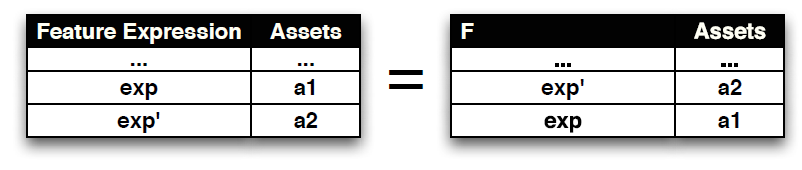
\includegraphics[width=1\textwidth, frame]{images/ChangeOrder}
\caption{Change Order (Taken from \cite{msclmt})}
\end{figure}

\pagebreak
\section{Templates for FM Refactoring}

\begin{figure}[H]
\centering
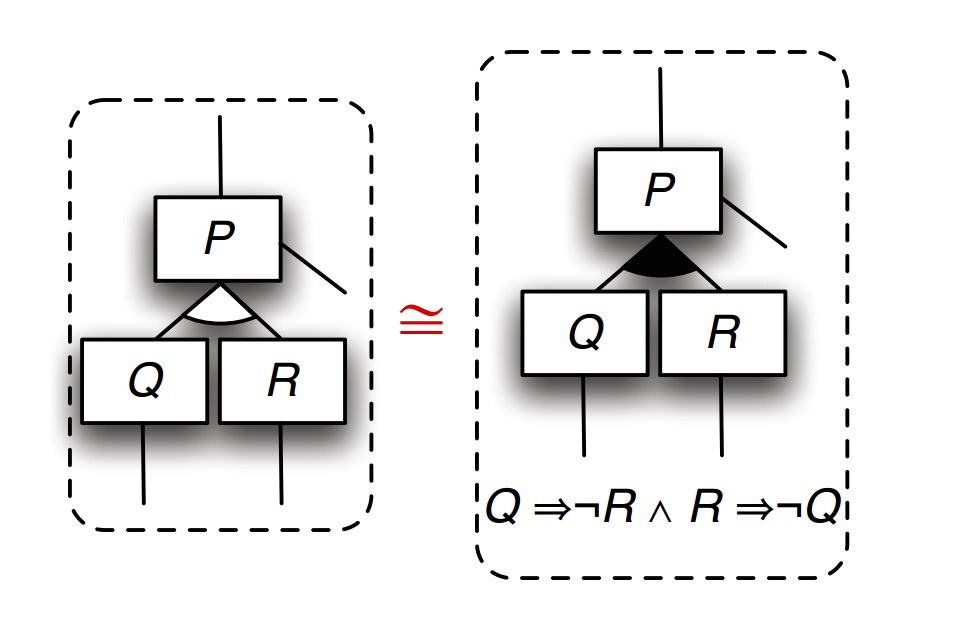
\includegraphics[width=1\textwidth, frame]{images/ReplaceAlternative}
\caption{Replace Alternative Equivalence Template (Taken from \cite{gttse})}
\end{figure}

\begin{figure}[H]
\centering
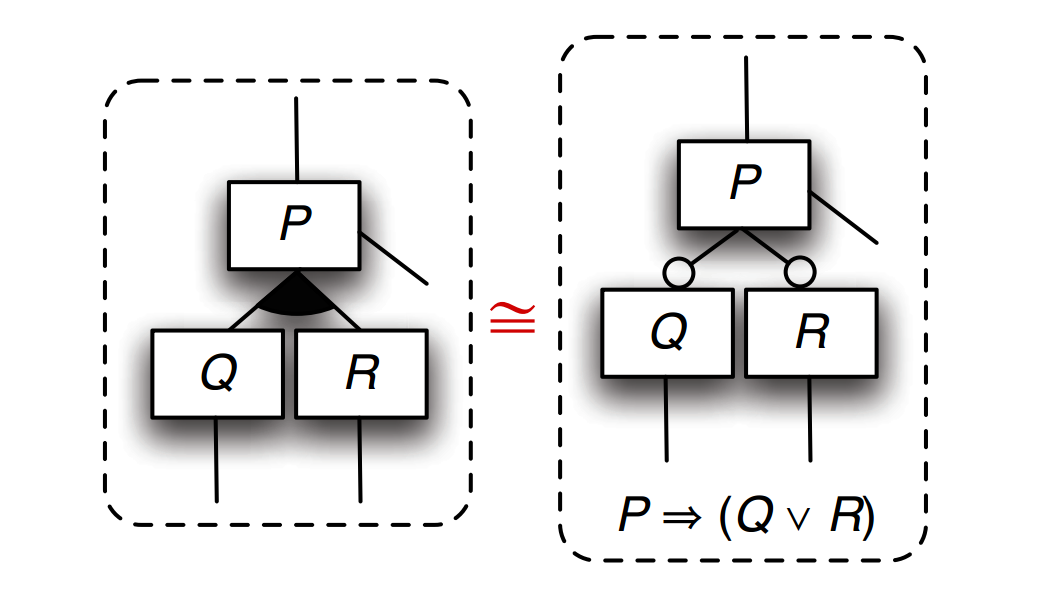
\includegraphics[width=0.9\textwidth, frame]{images/ReplaceOr}
\caption{Replace Or Equivalence Template (Taken from \cite{gttse})}
\end{figure}

\begin{figure}[H]
\centering
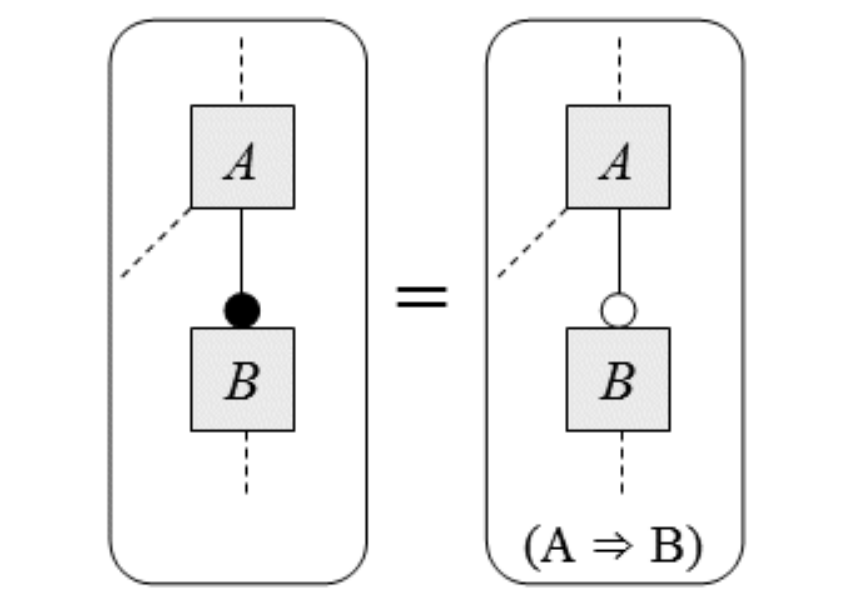
\includegraphics[width=0.8\textwidth, frame]{images/ReplaceMandatory}
\caption{Replace Mandatory (Taken from \cite{jucs})}
\end{figure}

\begin{figure}[H]
\centering
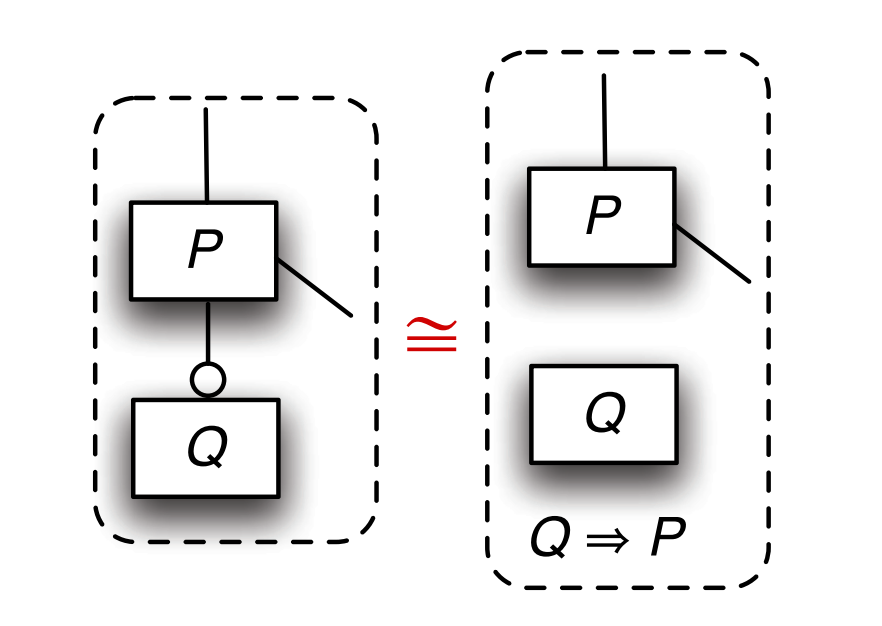
\includegraphics[width=0.8\textwidth, frame]{images/RemoveOptional}
\caption{Remove Optional Equivalence Template (Taken from \cite{gttse})}
\end{figure}

\begin{figure}[H]
\centering
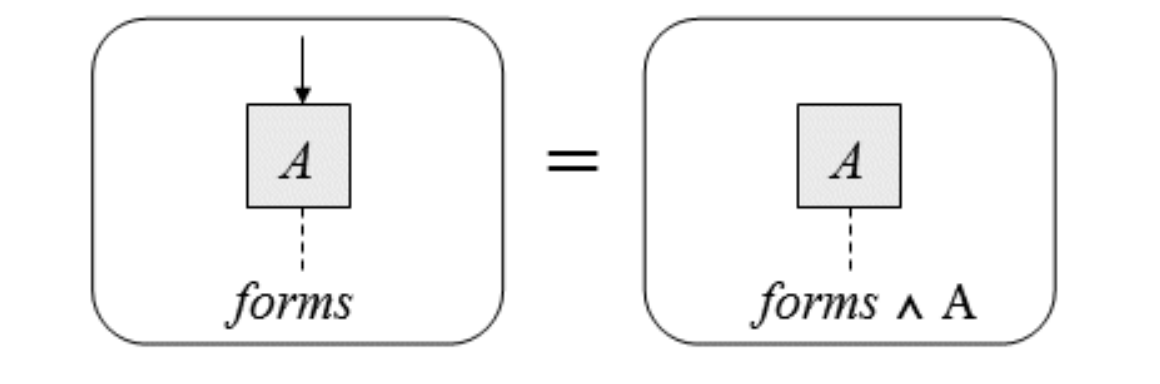
\includegraphics[width=1\textwidth, frame]{images/RemoveRoot}
\caption{Remove Root (Taken from \cite{jucs})}
\end{figure}

\begin{figure}[H]
\centering
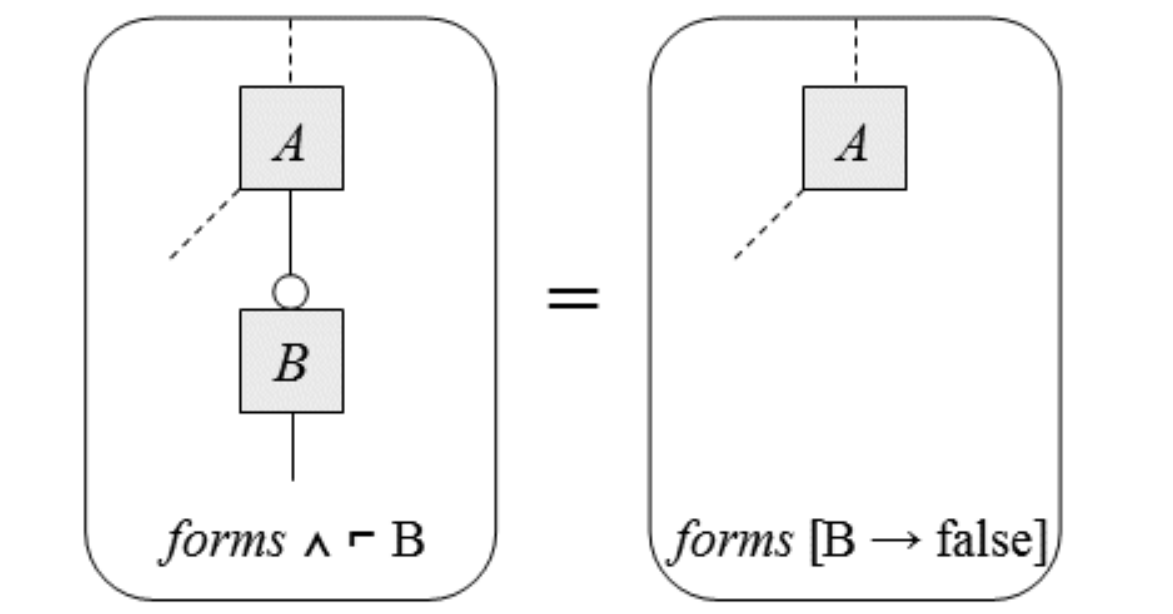
\includegraphics[width=1\textwidth, frame]{images/RemoveNode}
\caption{Remove Node (Taken from \cite{jucs})}
\end{figure}

\begin{figure}[H]
\centering
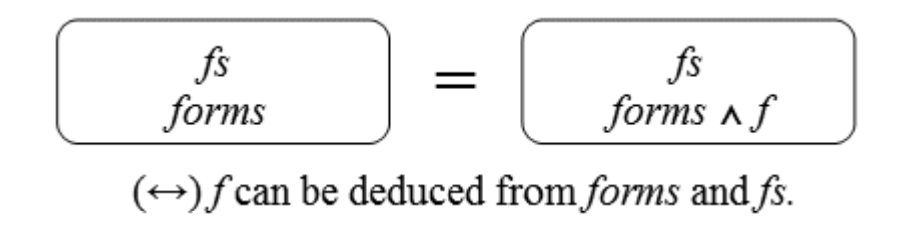
\includegraphics[width=0.9\textwidth, frame]{images/AddFormula}
\caption{Add Formula (Taken from \cite{jucs})}
\end{figure}

\pagebreak
\bibliographystyle{unsrt}
\bibliography{bibliography}
\end{document}